\section{Simultaneous position/force control}\label{sec:pos-force-control-exp}

This last example combines the explored methods from the previous experiments \ref{sec:2xminiJforce}-\ref{sec:pas-pos}. That means that the minimal CKC formulation explained in \ref{subsec:task-restrictions} is applied, and that the joint torques are computed for only the active joints as explained in \ref{subsec:passive-joints}. The rest of the control method is according to the dynamic HPFC control scheme presented in \ref{subsec:DHPFC}.

\begin{table}[h!]
    \centering
    \begin{tabular}{|c|c|c|}
        \hline
        & \textbf{Value} & \textbf{Unit}\\
        \hline \hline
        Number of obstacles & $3$ & \\
        Number of links & $6$ & \\
        $f_{F,d,3}$ & $1$ & $N$ \\
        $\theta_{t,d,3}$ & $0.1$ & $rad$ \\
        Force:$[K_{p}, K_{i}]$ & $[1, 0.005]$ &\\
        Position:$[K_{p}, K_{i}]$ & $[3, 0.005]$ &\\
        \hline
    \end{tabular}
    \caption{Simulation configuration for simultaneous position and force control experiment}
    \label{tab:p+f}
\end{table}

In this experiment, both position and force is controlled for the third contact point. More specifically, the angle of the link in contact with the third obstacle and the force this link applies to the obstacle are controlled. The exact desired values, as well as general simulation configurations for the experiment, are given in Table \ref{tab:p+f}. The values were chosen with the intuition of what would be achievable for the snake robot from its initial configuration. The control structure for the simulation is given in Figure \ref{fig:diag-pf}.

\begin{figure}
    \centering
    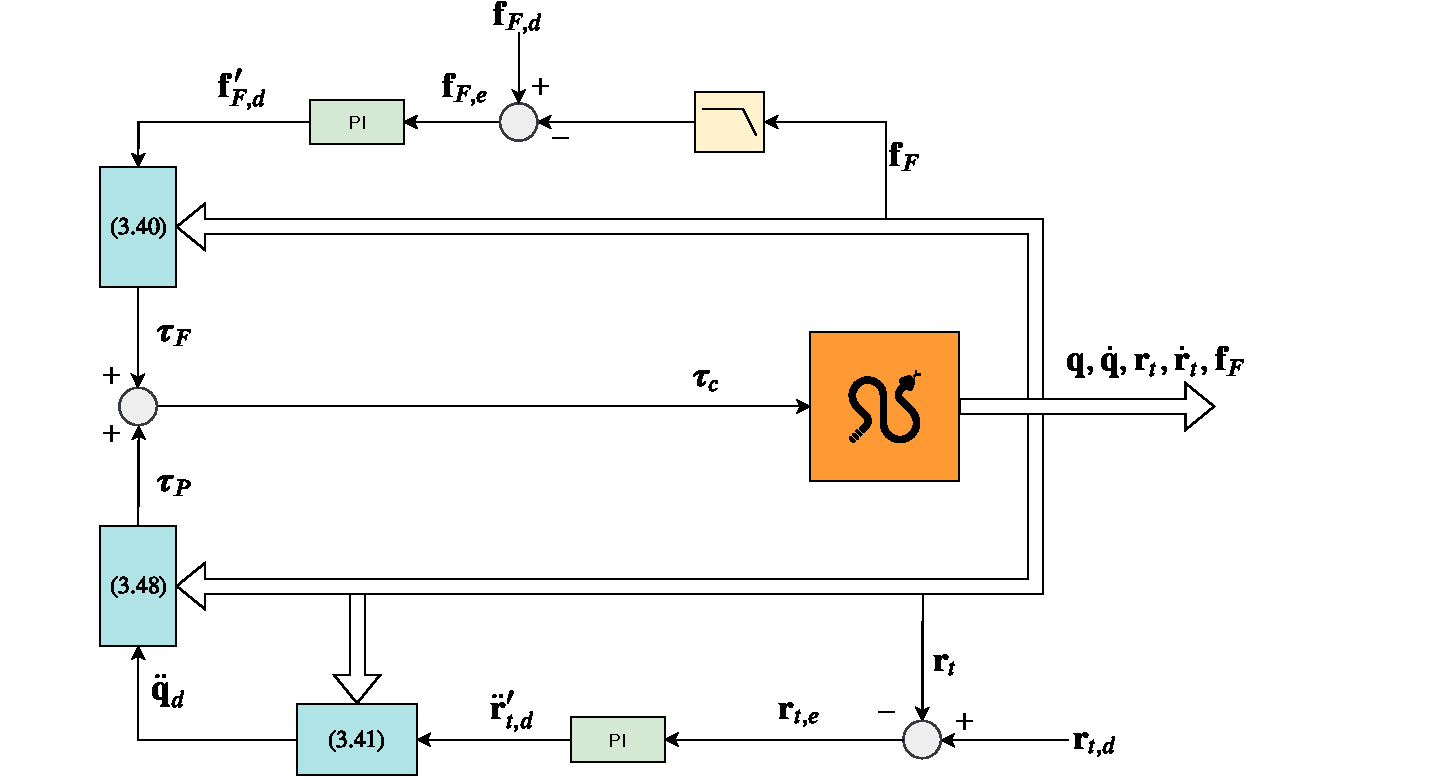
\includegraphics[trim=1cm 0cm 3cm 0cm, clip=true, width=\textwidth]{figures/experiments/control-diagrams/pf-control-diagram.pdf}
    \caption{Control diagram for dynamic HPFC}
    \label{fig:diag-pf}
\end{figure}
\newpage
The resulting contact link angle, contact force and joint torques are presented in Figure \ref{fig:p+f}. In this experiment, the torque values controlling the force are much smoother than the force signal, as opposed to the experiment in \ref{sec:2xminiJforce}. This is because the force sensor signal is filtered before it is sent to the controller. The force signal shown in the figure is unfiltered.

From Figure \ref{fig:p+f} it can also be seen that both the desired angle and force is reached. However, the angle takes longer to reach its reference and does have a slightly irregular trajectory. Both this and the very sensitive force signals can be a result of the nature of the simulator used.
%In addition, since the movements are all over slow, the snake robot ends up stopping and starting frequently, forcing it to also frequently overcome its inertia and suddenly start moving. \hl{yay or nay?}

From the input torque plot in Figure \ref{fig:p+f} it can be observed that the commanded torques $\tau_1$, $\tau_2$ and $\tau_3$ are used only for the position control since they are smoother, whereas $\tau_4$ and $\tau_5$ are used for both position and force control. The idea of Yoshikawa \cite{yoshikawa1987dynamic} is that this can still yield successful HPFC given that the dynamical model is correct. The position and force loops are included to compensate for possible modeling errors.

\begin{figure}
    \centering
    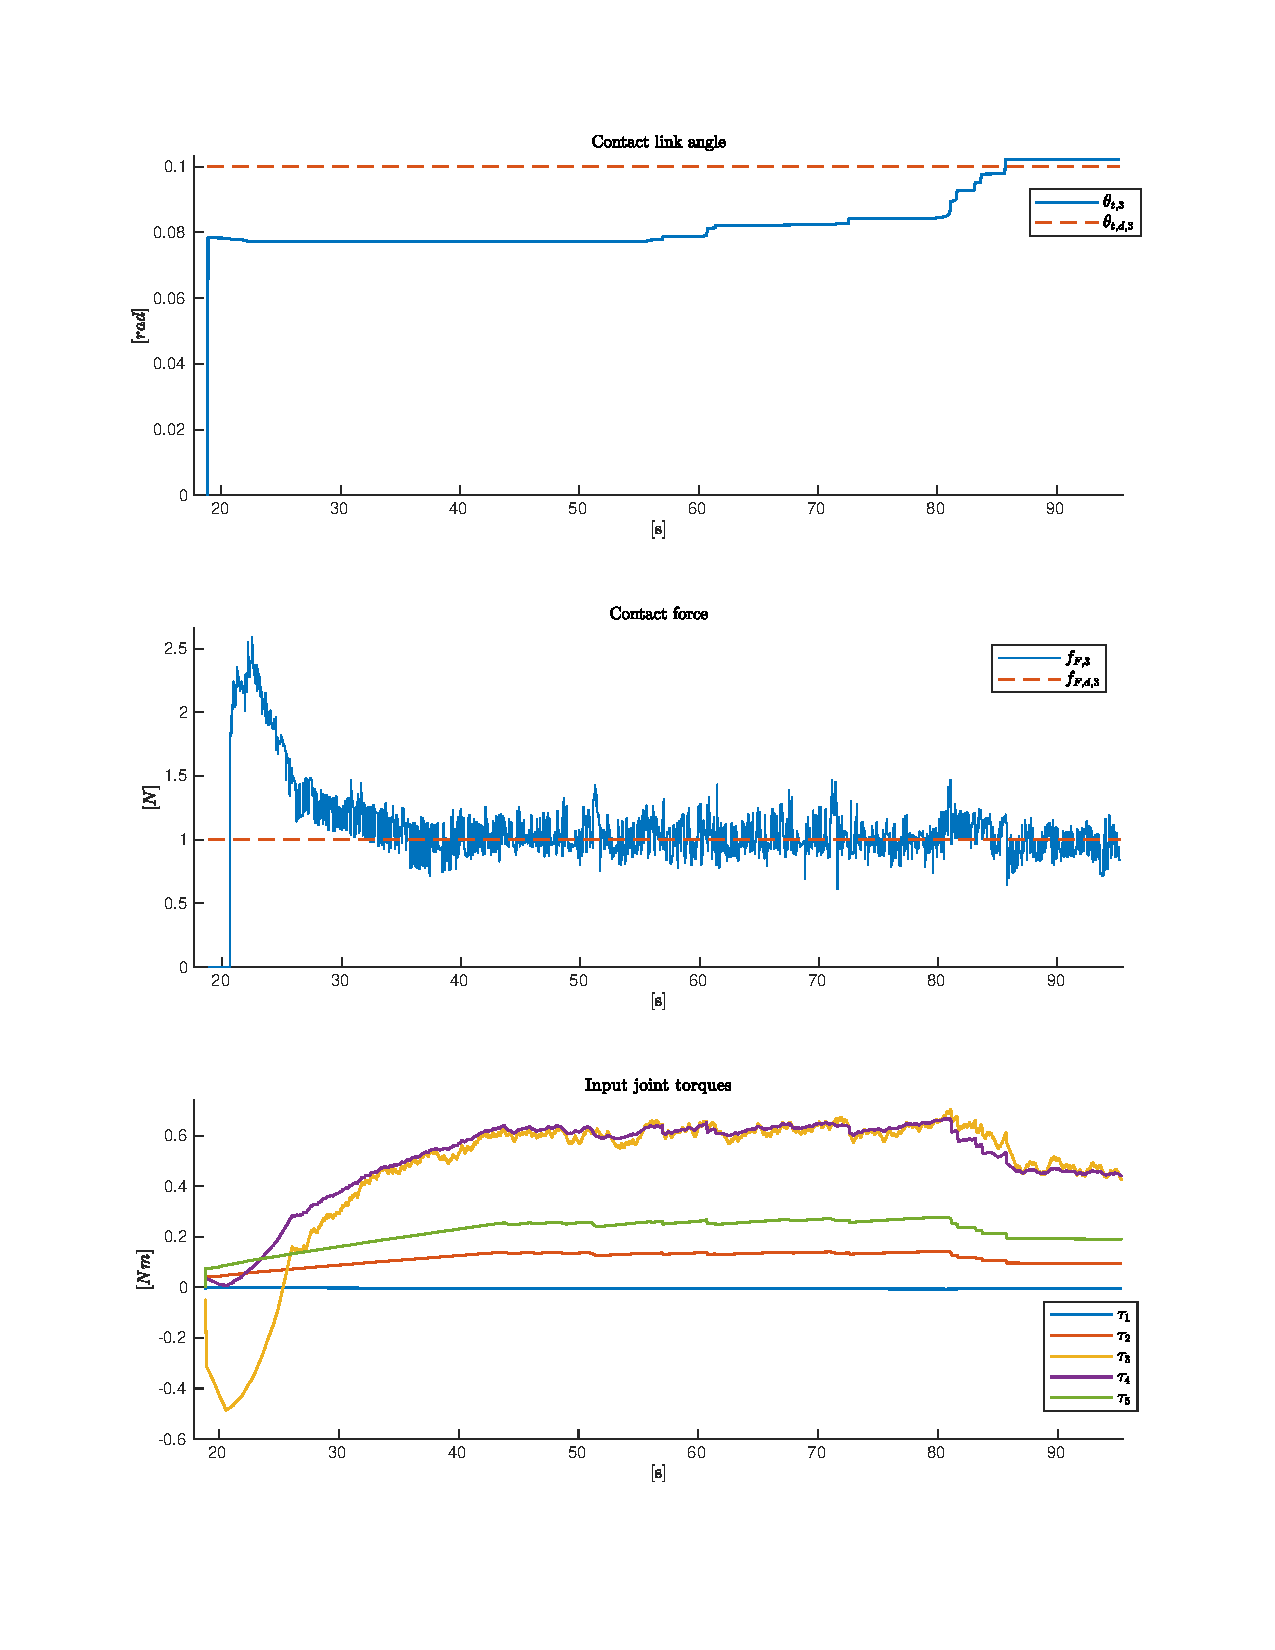
\includegraphics[trim=2.1cm 2.1cm 2.1cm 2.1cm, clip=true, width=\textwidth]{figures/experiments/pos+f/pf-ref-3.pdf}
    \caption{Results from simultaneous force and position control}
    \label{fig:p+f}
\end{figure}